\chapter*{Úvod} % SEM NESAHEJTE!
\addcontentsline{toc}{chapter}{Úvod} % SEM NESAHEJTE!
\markboth{Úvod}{Úvod}
\section{Cíl projektu}
Cílem projektu je realizovat dva typy měření:

První měření se zabývá empirickým modelem. Jedna anténa je pevně umístěna na stojanu, zatímco druhá simuluje mobilní terminál. Cílem je získat závislost ztrát na poloze obou antén ve statickém prostředí pro úzkopásmový přenos. Nejjednodušší způsob je zaznamenávat úroveň při pohybu terminálu konstantní rychlostí po přímce směrem k/od pevné antény.

Druhé měření se zabývá měřením úniků způsobených vícecestným šířením. Obě antény jsou pevně umístěny na stojanech v dostatečné vzdálenosti (pro dané prostředí) na přímou viditelnost. Časový průběh přijímané úrovně úzkopásmového signálu je zaznamenán po dobu cca jedné minuty pro minimálně tři případy: v prvním neovlivňujte okolní prostředí (resp. spoj), ve druhém se naopak pokuste co nejvíce dynamicky spoj narušovat (např. pohybem členů týmu zastiňujícím přímou viditelnost mezi anténami) a ve třetím se pokuste dynamiku změn ještě zvýšit a zároveň dosáhnout trvalého zastínění spoje (za tím účelem můžete i změnit polohu antén). 


\section{Oficiální zadání}
\begin{enumerate}
\item Realizovat měření v terénu za účelem lepšího porozumění podstatě úniků mobilního spoje v pásmu UHF (300 MHz - 3 GHz) v různých prostředích. 
\item Využít měřená data pro odvození empirického modelu závislosti ztrát na vzdálenosti. 
\item Na základě výsledků měření statisticky analyzovat úniky způsobené vícecestným šířením. 
\end{enumerate}

\section{Použité vybavení}
Během měření bylo použito následující vybavení:
\begin{itemize}
    \item USB SDR Adalm Pluto pro vysílání, 
    \item Přenosný přijímač Rohde \& Schwarz PR100, 
    \item 2x všesměrová anténa se stojanem, 
    \item Mobilní telefon pro dokumentaci měření,
    \item Laserový dálkoměr Nikon Prostaff S 6x21 7.5
\end{itemize}

\begin{figure}[h!]
    \centering
    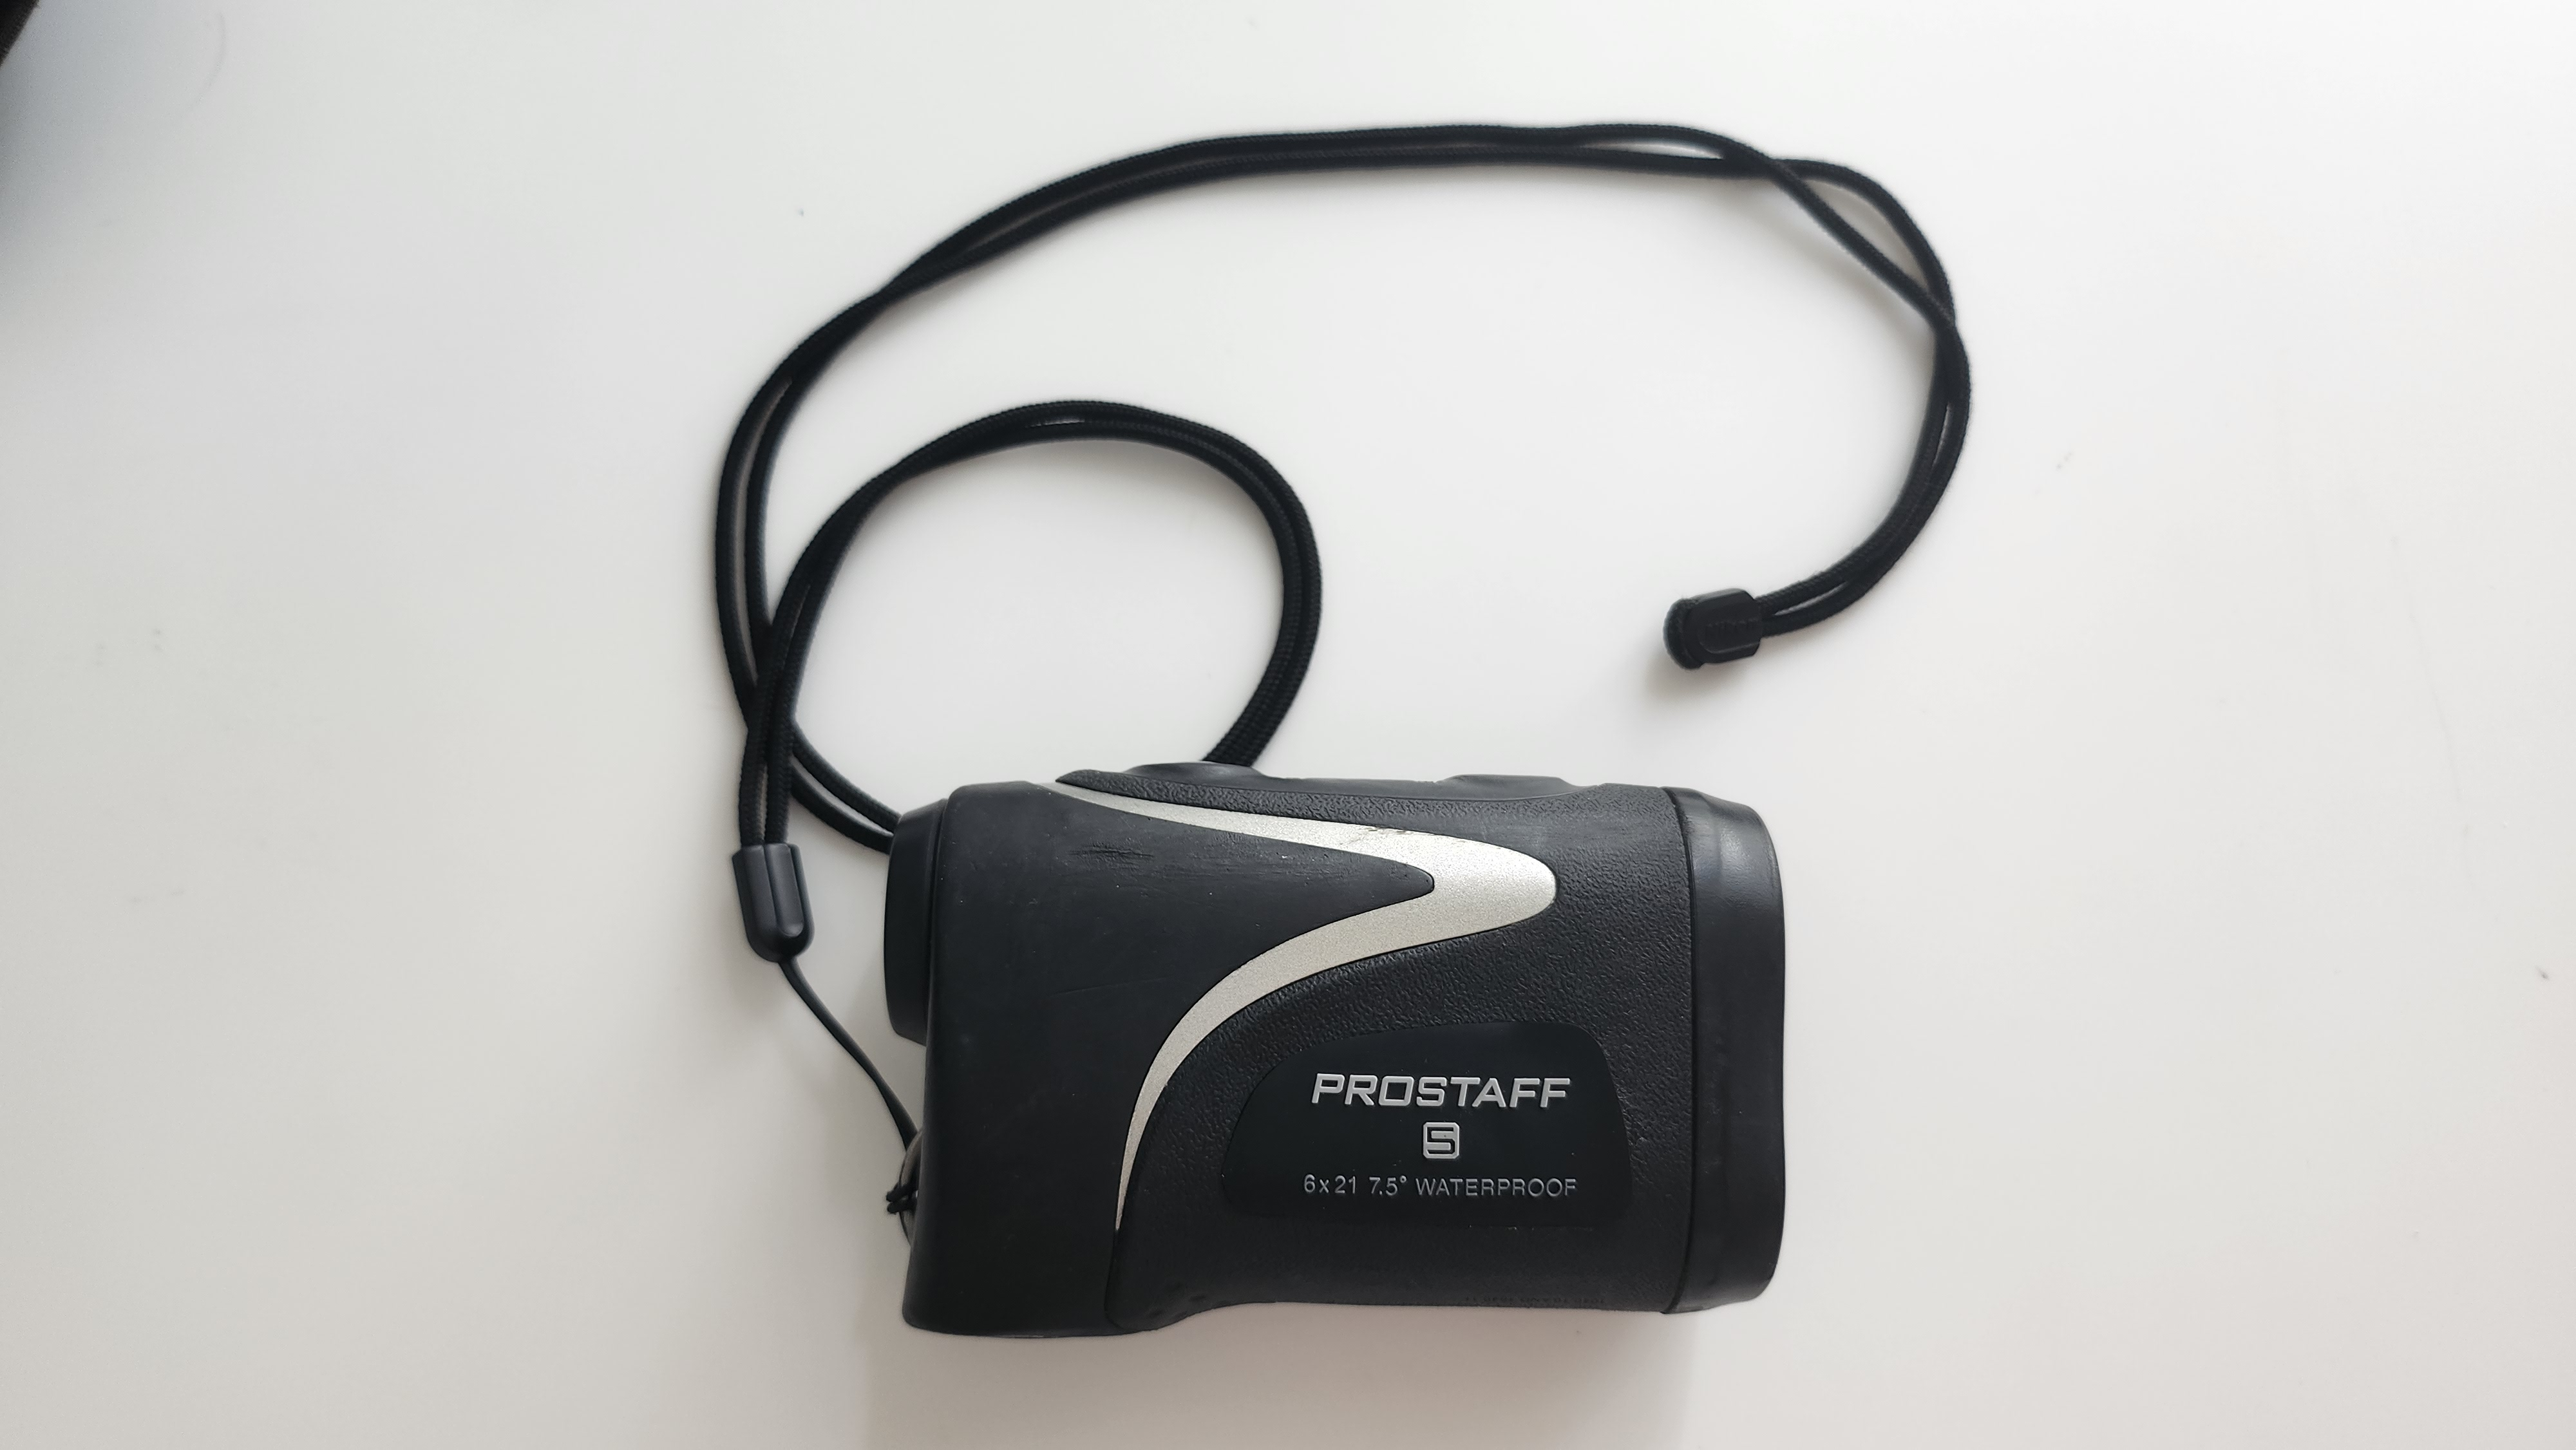
\includegraphics[scale=0.075]{img/dalkomer.jpg}
    \caption{Laserový dálkoměr Nikon Prostaff S 6x21 7.5}
    \label{fig:my_label}
\end{figure}

\begin{figure}[h!]
    \centering
    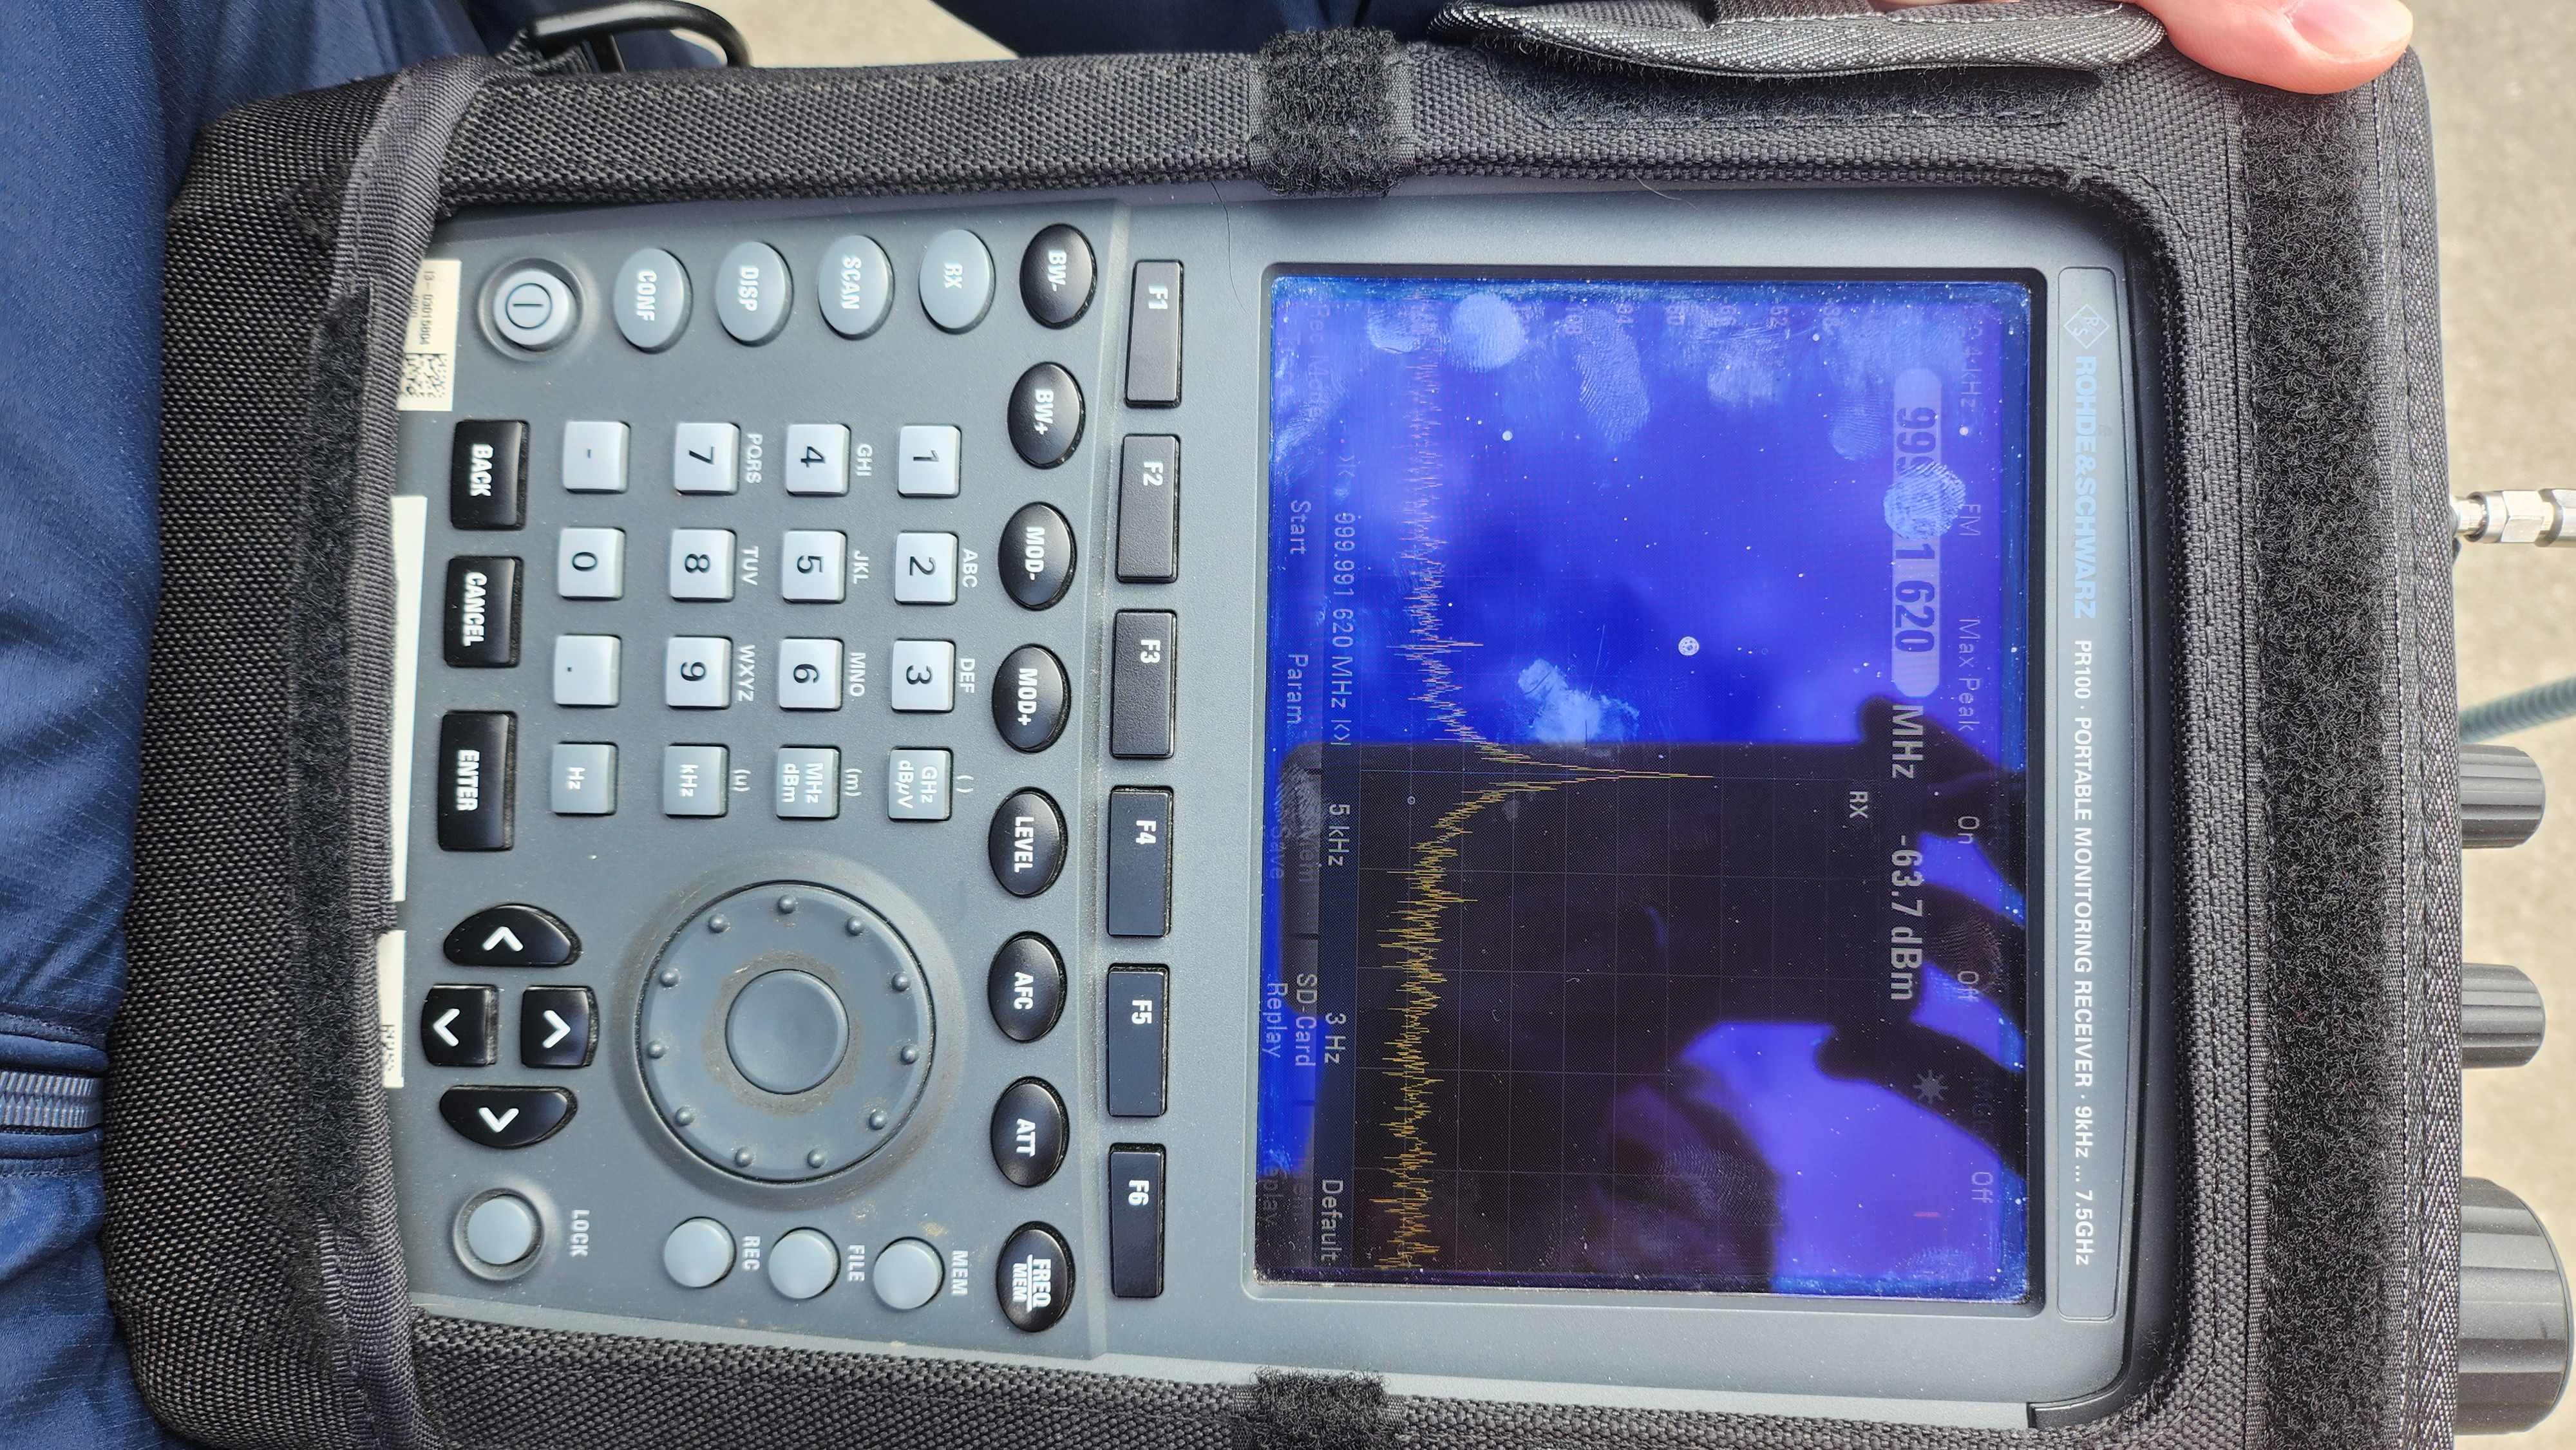
\includegraphics[angle=90,scale=0.06]{img/prijimac1.jpg}
    \caption{Přenosný přijímač Rohde \& Schwarz PR100 s krytem v terénu}
    \label{fig:my_label}
\end{figure}

\begin{figure}[h!]
    \centering
    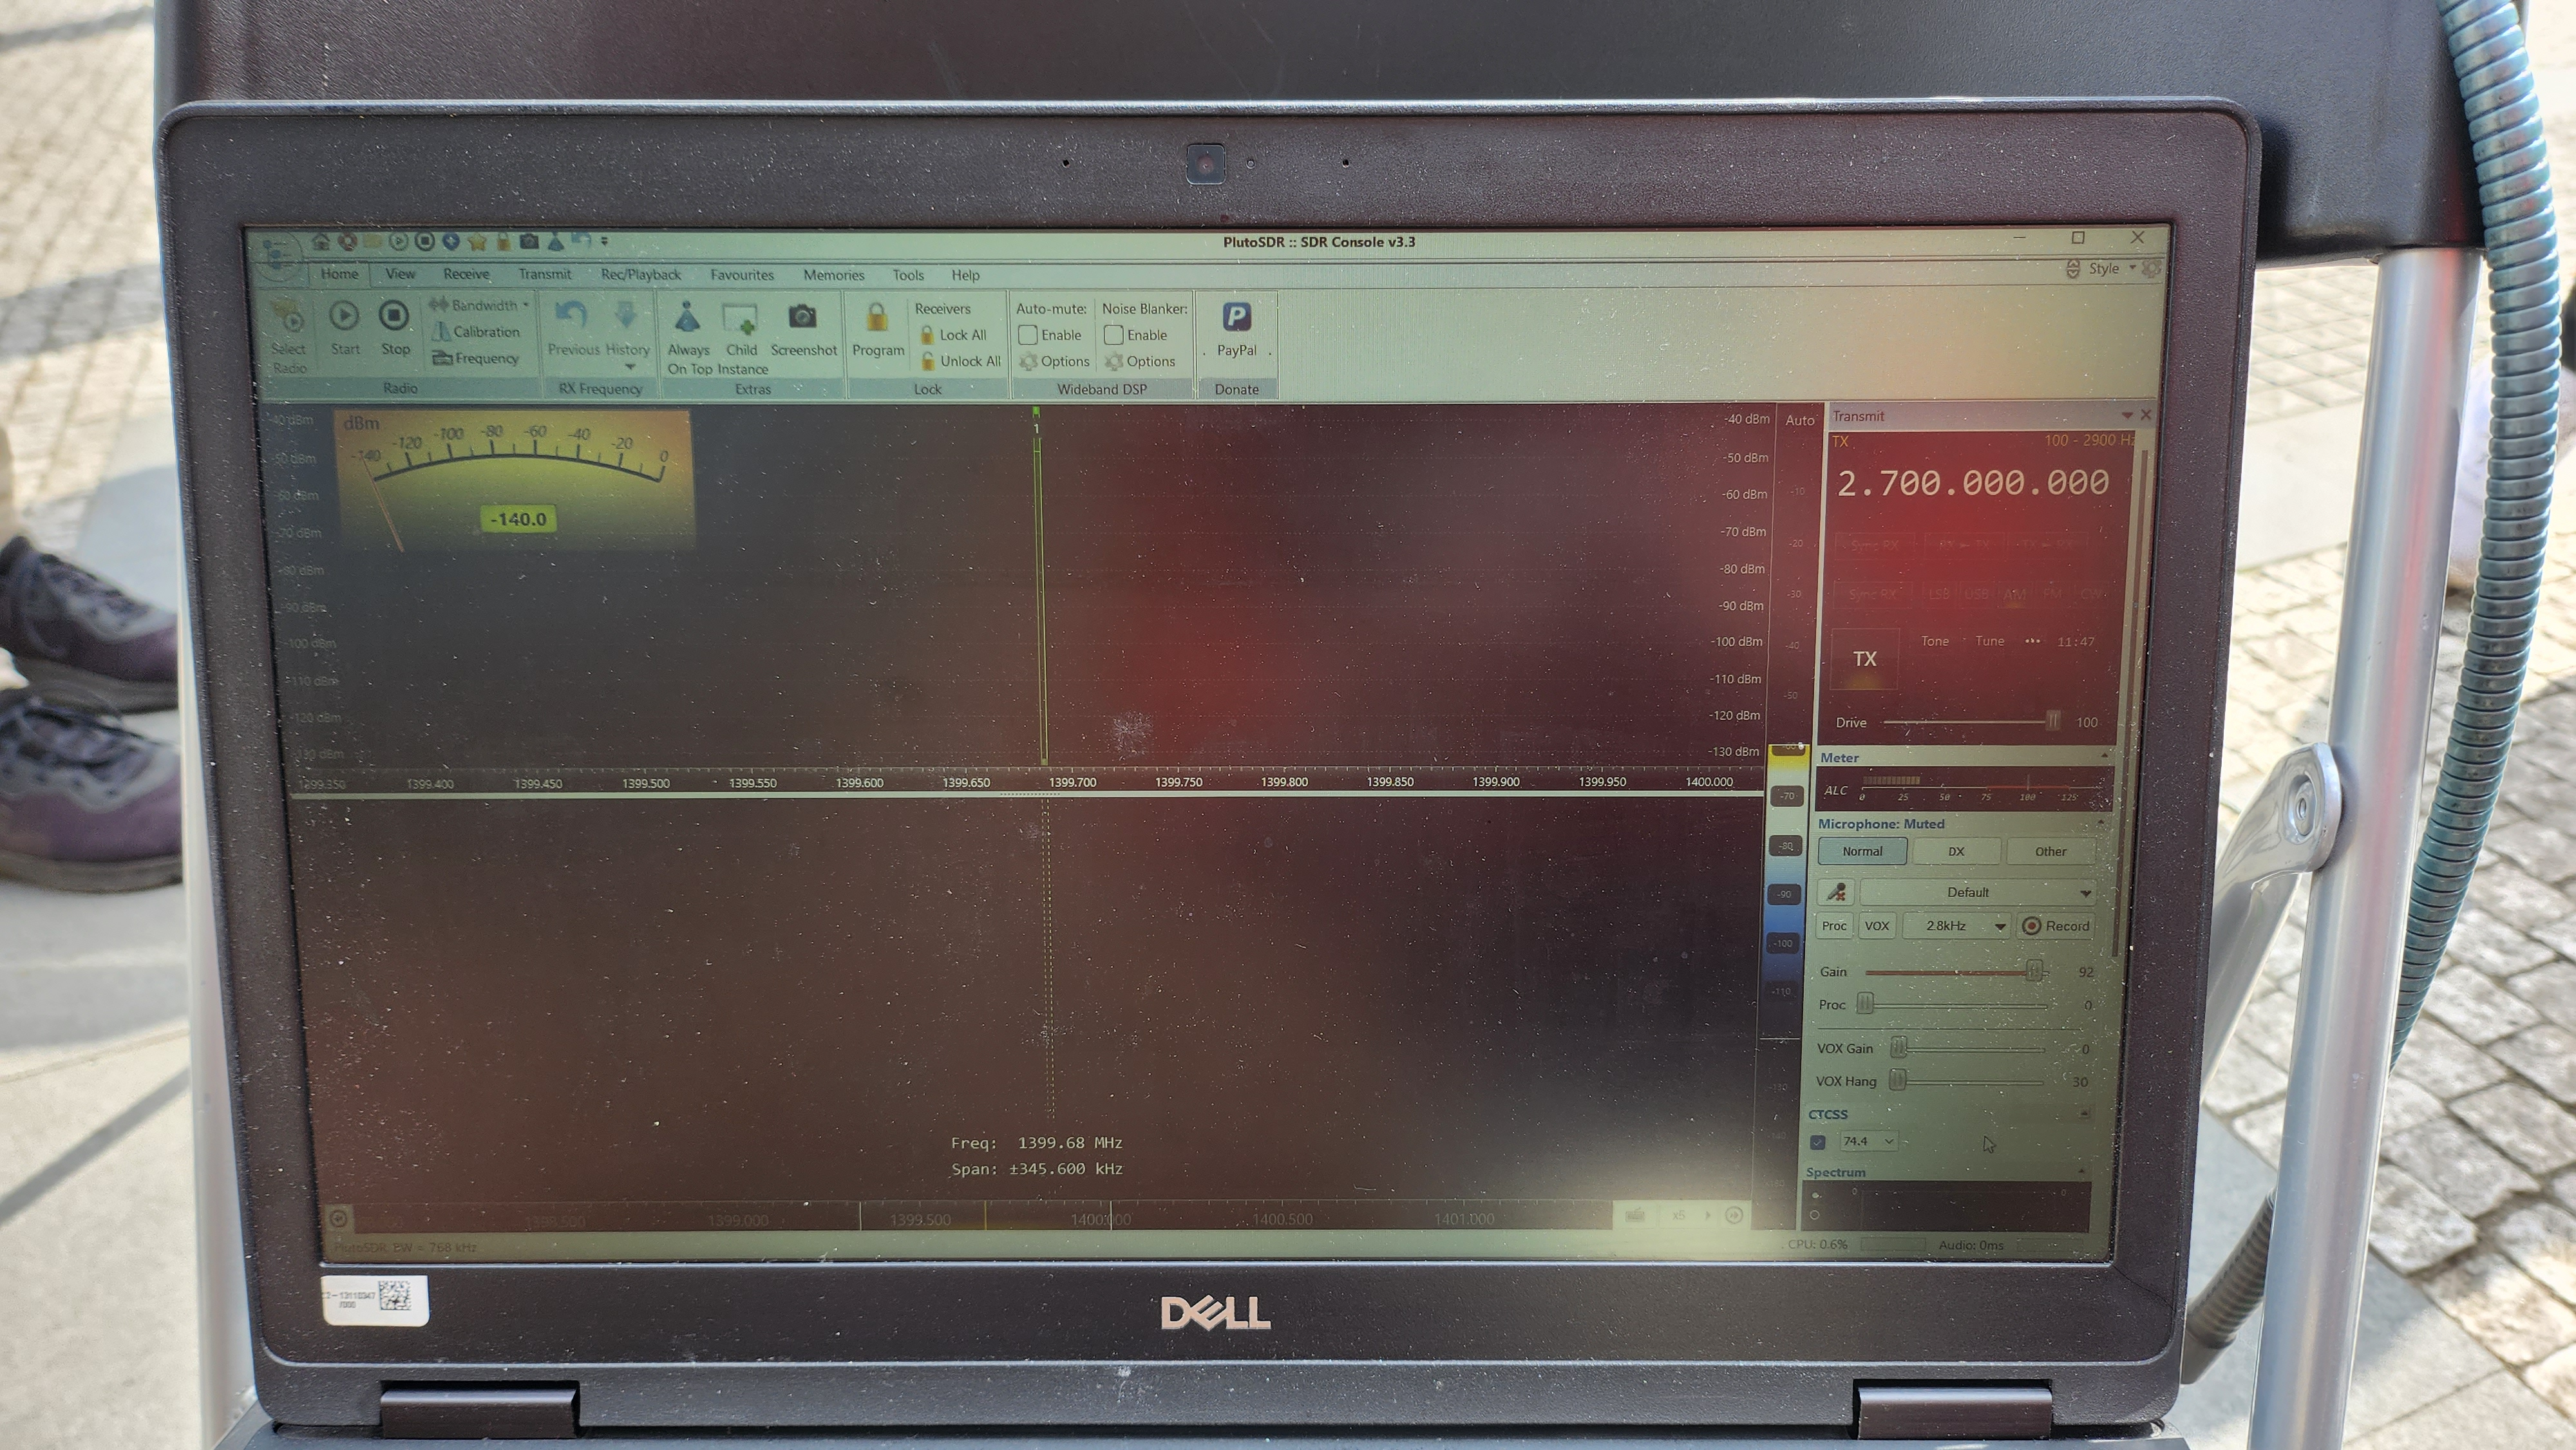
\includegraphics[scale=0.075]{img/notebook.jpg}
    \caption{Software pro vysílání běžící na notebooku v terénu}
    \label{fig:my_label}
\end{figure}

\begin{figure}[h!]
    \centering
    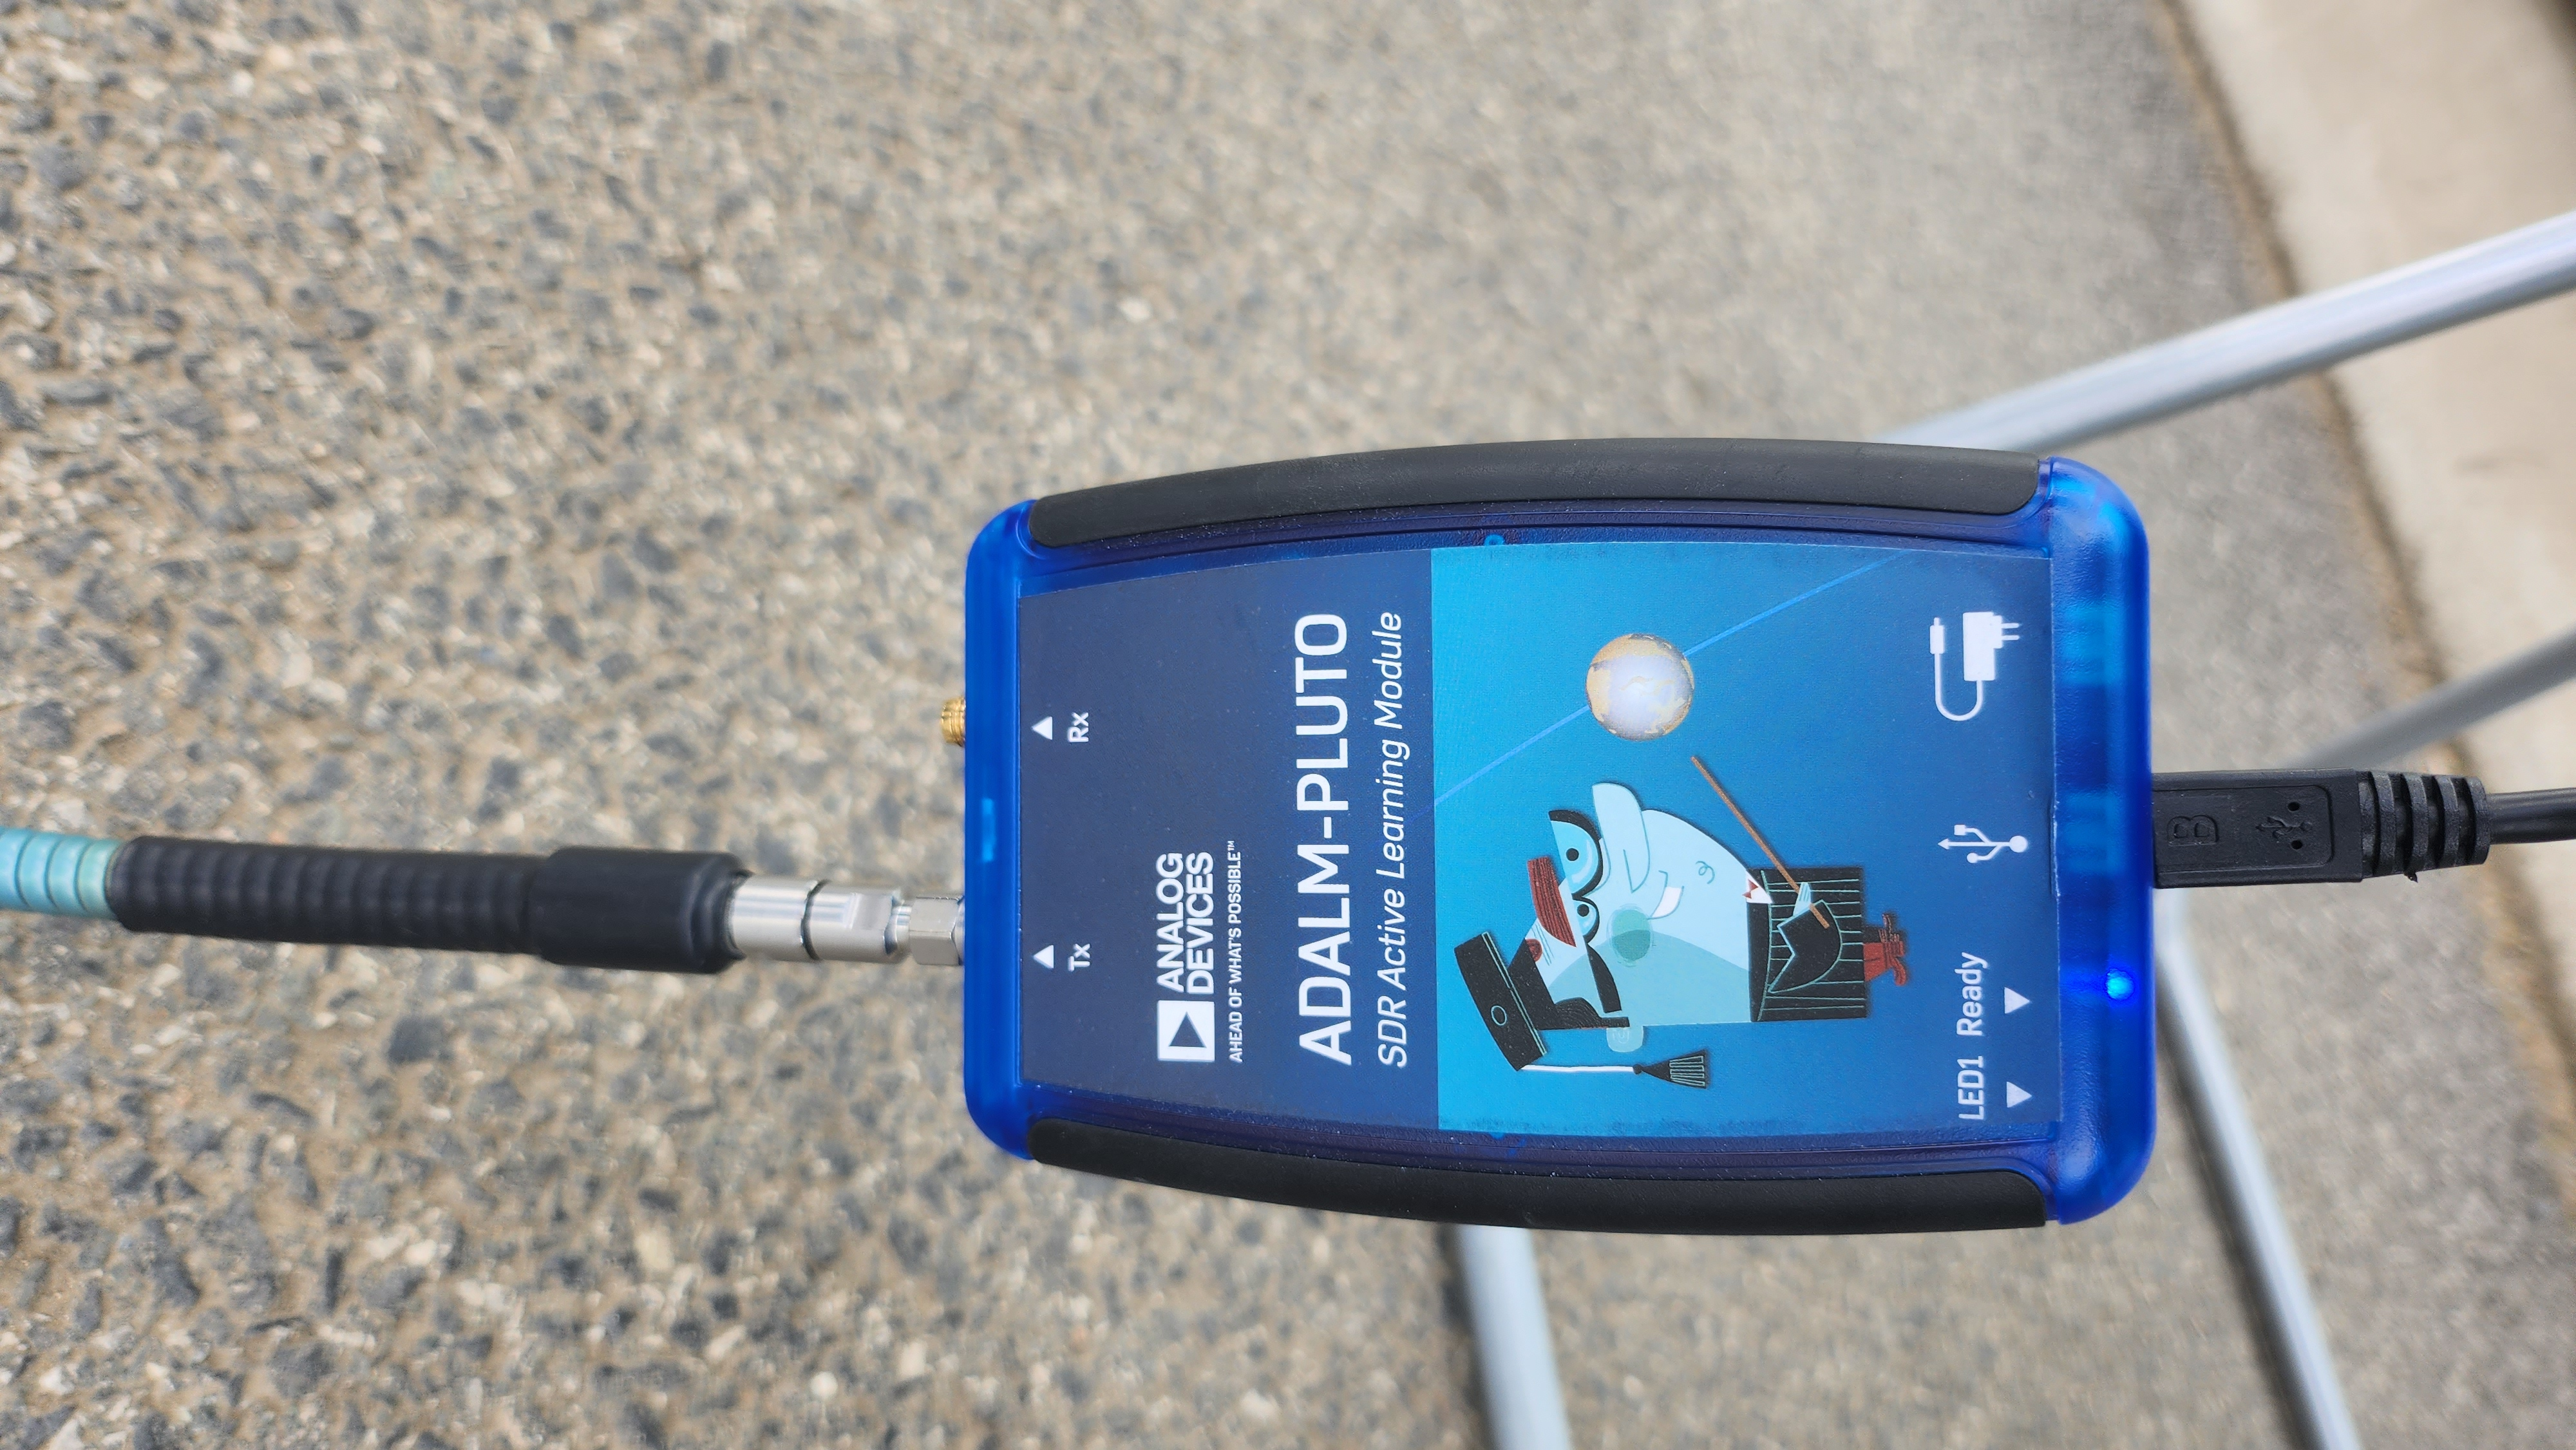
\includegraphics[angle=270,scale=0.06]{img/SDR-pluto.jpg}
    \caption{SDR Adalm-Pluto}
    \label{fig:my_label}
\end{figure}

\begin{figure}[h!]
    \centering
    \includegraphics[angle=270,scale=0.06]{img/antena_vysilaci.jpg}
    \caption{Vysílací anténa upevněná na stojanu během měření}
    \label{fig:my_label}
\end{figure}

\section{Paramtery pro měření:}
\begin{itemize}
    \item Frekvence: 1 GHz
    \item Výška, ve které byly umístěny antény během měření úniků způsobených vícecestným šířením: 1,4 m
    \item Výška, ve které byly umístěny antény při měření I (emperický model): 1,7 m 
    \item Polarizace: Vertikální
\end{itemize}

